\documentclass[tikz,border=0pt]{standalone}
\usepackage[utf8]{inputenc}
\usepackage[T1]{fontenc}
\usepackage{lmodern}
\usepackage{amsmath,amssymb}
\usetikzlibrary{arrows.meta,positioning,fit,calc,backgrounds,shapes.geometric,decorations.pathreplacing}
\definecolor{navy}{HTML}{163A5F}
\definecolor{blue}{HTML}{2C6EAF}
\definecolor{lightblue}{HTML}{EAF2F8}
\definecolor{midblue}{HTML}{CFE1F2}
\definecolor{graytext}{HTML}{4A5560}
\definecolor{lightgray}{HTML}{F4F6F8}
\definecolor{green}{HTML}{3C8D73}
\definecolor{lightgreen}{HTML}{E8F5EF}
\definecolor{red}{HTML}{B24A4A}
\definecolor{lightred}{HTML}{FBEDEE}
\tikzset{
  title/.style={font=\sffamily\bfseries\fontsize{18}{20}\selectfont,text=navy,anchor=west},
  subtitle/.style={font=\sffamily\bfseries\fontsize{11}{13}\selectfont,text=navy},
  body/.style={font=\sffamily\fontsize{9.2}{11}\selectfont,text=graytext,align=left},
  small/.style={font=\sffamily\fontsize{8}{9.4}\selectfont,text=graytext,align=left},
  tinylabel/.style={font=\sffamily\fontsize{7.2}{8.4}\selectfont,text=graytext},
  panel/.style={rounded corners=3pt,draw=midblue,fill=white,line width=0.6pt},
  box/.style={rounded corners=2pt,draw=midblue,fill=lightblue,line width=0.6pt},
  worker/.style={rounded corners=2pt,draw=blue,dashed,line width=0.7pt,fill=white},
  task/.style={rounded corners=2pt,draw=blue,fill=lightblue,minimum width=0.85cm,minimum height=0.55cm,font=\sffamily\bfseries\small,text=navy},
  file/.style={draw=blue,fill=white,minimum width=0.55cm,minimum height=0.42cm,font=\sffamily\small,text=navy},
  arr/.style={-{Stealth[length=2.4mm,width=1.8mm]},draw=blue,line width=0.9pt},
  arrthin/.style={-{Stealth[length=2mm,width=1.5mm]},draw=blue,line width=0.7pt},
  arrred/.style={-{Stealth[length=2mm,width=1.5mm]},draw=red,dashed,line width=0.8pt},
  arrgreen/.style={-{Stealth[length=2mm,width=1.5mm]},draw=green,dotted,line width=1pt}
}
\begin{document}

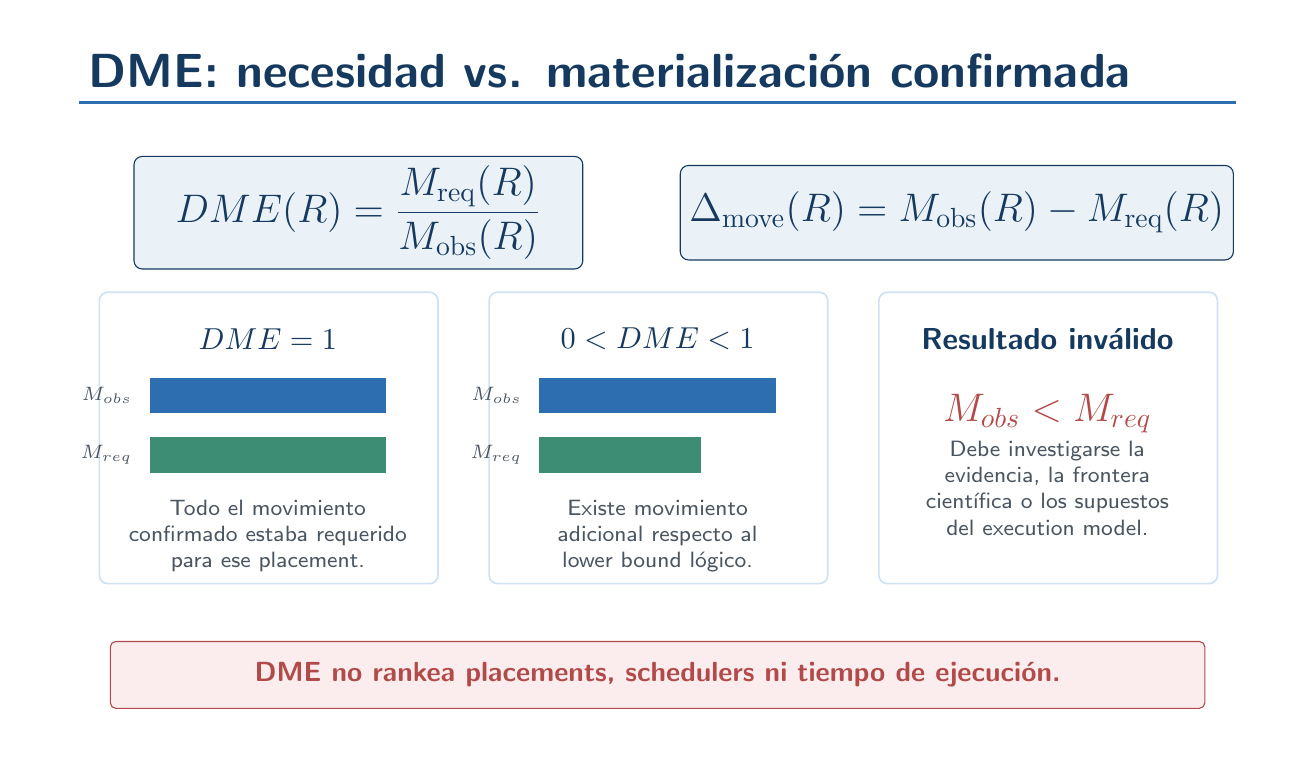
\begin{tikzpicture}[x=1cm,y=1cm]
\path[use as bounding box] (0,0) rectangle (16,9);
\node[title] at (0.65,8.45) {DME: necesidad vs. materialización confirmada};
\draw[blue,line width=1pt] (0.65,8.05)--(15.35,8.05);
\node[rounded corners=3pt,draw=navy,fill=lightblue,minimum width=5.7cm,minimum height=1.2cm,font=\sffamily\bfseries\Large,text=navy] at (4.2,6.65) {$DME(R)=\dfrac{M_{\mathrm{req}}(R)}{M_{\mathrm{obs}}(R)}$};
\node[rounded corners=3pt,draw=navy,fill=lightblue,minimum width=5.7cm,minimum height=1.2cm,font=\sffamily\bfseries\Large,text=navy] at (11.8,6.65) {$\Delta_{\mathrm{move}}(R)=M_{\mathrm{obs}}(R)-M_{\mathrm{req}}(R)$};

\node[panel,minimum width=4.3cm,minimum height=3.7cm,anchor=north west] at (0.9,5.65) {};
\node[subtitle] at (3.05,5.05) {$DME=1$};
\fill[blue] (1.55,4.1) rectangle (4.55,4.55);
\fill[green] (1.55,3.35) rectangle (4.55,3.8);
\node[tinylabel,anchor=east] at (1.45,4.33) {$M_{obs}$};
\node[tinylabel,anchor=east] at (1.45,3.58) {$M_{req}$};
\node[small,text width=3.6cm,align=center] at (3.05,2.55) {Todo el movimiento confirmado estaba requerido para ese placement.};

\node[panel,minimum width=4.3cm,minimum height=3.7cm,anchor=north west] at (5.85,5.65) {};
\node[subtitle] at (8.0,5.05) {$0<DME<1$};
\fill[blue] (6.5,4.1) rectangle (9.5,4.55);
\fill[green] (6.5,3.35) rectangle (8.55,3.8);
\node[tinylabel,anchor=east] at (6.4,4.33) {$M_{obs}$};
\node[tinylabel,anchor=east] at (6.4,3.58) {$M_{req}$};
\node[small,text width=3.6cm,align=center] at (8.0,2.55) {Existe movimiento adicional respecto al lower bound lógico.};

\node[panel,minimum width=4.3cm,minimum height=3.7cm,anchor=north west] at (10.8,5.65) {};
\node[subtitle] at (12.95,5.05) {Resultado inválido};
\node[font=\sffamily\bfseries\Large,text=red] at (12.95,4.1) {$M_{obs}<M_{req}$};
\node[small,text width=3.6cm,align=center] at (12.95,3.15) {Debe investigarse la evidencia, la frontera científica o los supuestos del execution model.};

\node[rounded corners=2pt,draw=red,fill=lightred,minimum width=13.9cm,minimum height=0.85cm,font=\sffamily\bfseries,text=red] at (8,0.78) {DME no rankea placements, schedulers ni tiempo de ejecución.};
\end{tikzpicture}
\end{document}
